\documentclass[catalan, a4paper, 12pt, titlepage]{article}
\usepackage{babel}
\usepackage{graphicx}
\usepackage{mathptmx}
\renewcommand{\baselinestretch}{1.5}
%\usepackage{isolatin1}

%tikz
\usepackage{tikz}
\usetikzlibrary{mindmap}

\title{Una programació didàctica de \\
gestió de bases de dades\\
	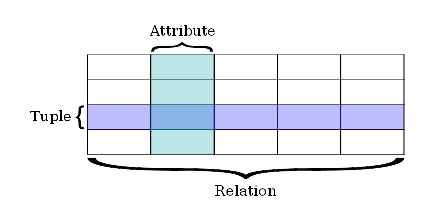
\includegraphics[width=10cm]{database.eps}
	}

\author{
	Jaume Barceló Vicens\\
	DNI 43135949R\\
	Professors d'ensenyament secudari (0590)\\
	Especialitat informàtica}

\date{
	Família professional informàtica \\
	Cicle formatiu de grau superior d’Administració de Sistemes Informàtics en Xarxa\\
	Mòdul professional de gestió de bases de dades\\
	Codi 0372 170h (+90h d'anglès)}

\begin{document}

\maketitle

\tableofcontents 

\section{Introducció}

Aquesta és la programació didàctica del mòdul ``Gestió de bases de dades'' (codi 0372) del cicle fomatiu de ``Tècnic superior en administració de sistemes i xarxes'' que s'imparteix al CIFP Francesc de Borja Moll el curs escolar 2020-2021.

Aquesta programació tracta de reflexar l'experiència de l'impartició d'aquest mateix mòdul durant el curs 2019-2020. A més, aquesta programació didàctica es presenta com una guia oberta i flexible, sobre la que es poden fer tants canvis com siguin necessaris per adaptar-se a la realitat del grup d'alumnes i del curs en general.

Aquesta programació s'ha desenvolupat tenint en compte la següent normativa estatal:
\begin{itemize}
	\item Llei Orgànica 2/2006, de 3 de maig, d'Educació, que assenyala que el Gobierno de España, prèvia consulta a les comunitats autònomes, establirà les titulacions de formació professional i els aspectes bàsics del currículum.
	\item Llei Orgànica, 8/2013, de 9 de desembre per a la millora de la qualitat educativa i que modifica la LOE.
	\item Llei Orgànica 5/2002, de 19 de juny, de les Qualificacions i de la Formació Professional, que posa en marxa el Sistema Nacional de Qualificacions i Formació professional, desenvolupada pel Reial Decret 1128/2003, de 5 de setemebre, modificat pel Reial Decret 1416/2005, de 25 de novembre, sobre el Catàleg Nacional de Qualificacions Professionals.
	\item Reial Decret 1147/2011, de 29 de juliol, pel qual s'estableix l'ordenació general de la formació professional basada en el Catàleg Nacional de Qualificacions Professionals.
	\item Reial Decret 1629/2009, de 30 d'octubre, pel que s'estableix el títol de ``Tècnic Superior en Administració de Sistemes Informàtics en Xarxa'' i es fixen els seus ensenyaments mínims.
	\item Ordre EDU / 392/2010, de 20 de gener, per la qual s'estableix el currículum del cicle formatiu de grau superior corresponent al títol de ``Tècnic Superior en Administració de Sistemes Informàtics en Xarxa''.
\end{itemize}

En l'àmbit autonòmic considerem la següent normativa:
\begin{itemize}
	\item Decret 91/2012, de 23 de novembre, pel qual s'estableix l'ordenació general de la formació professional del sistema educatiu en el sistema integrat de formació professional a les Illes Balears.
	\item Ordre de la consellera d'Educació i Cultura de 13 de juliol de 2009 per la qual es regula l'organització i el funcionament dels cicles formatius de formació professional del sistema educatiu que s'imparteixen d'acord amb la Llei orgànica 2/2006, de 3 de maig, d'educació, a les Illes Balears, en la modalitat d'ensenyament presencial.
	\item Resolució del conseller d'Educació i Universitat de 18 d'abril de 2018 per la qual s'estableix el calendari escolar del curs 2018-2019 per als centres docents no universitaris de la comunitat autònoma de les Illes Balears.
\end{itemize}

Finalment, en l'àmbit del centre, considerem la següent normativa:
\begin{itemize}
	\item Projecte educatiu de centre (PEC) que planteja les intencions educatives i organitzatives del CIFP: las seva missió, visió i valors. I que inclou com a annexes el projecte lingüístic, el reglament d'organització i funcionament i la concreció curricular del centre.
\end{itemize}

\section{Contextualització}

Aquesta programació didàctica és per al mòdul Gestió de Bases de Dades del Cicle Formatiu de Grau Superior d'Administració de Sistemes Informàtics i Xarxes del Centre Integrat de Formació Professional Francesc de Borja Moll. 

A la comunitat Autònoma de les Illes Balears, la tipologia dels centres integrats ha estat reconeguda a partir de la Resolución del conseller d'educació i universitat de 24 de maig de 2018 per la qual es determina la tipologia dels centres docents públics no universitaris.

El centra es crea el curs 2019-20 amb estudis de doble torn i comparteix espais amb l'IES Nou Llevant. A més d'Inforàtica, hi trobam estudis de Comerç i màrqueting, imatge Personal, sanitat i Seguretat i medi ambient.



\section{Objectius generals}

Els objectius generals estableixen les capacitats que s'espera que els alumnes hagin assolit a final de curs. Segons el títol de tècnic superior en administració de sistemes informàtics en xarxa, s'estableixen els següents objectius.

1. Analitzar l'estructura del programari de base, comparant les característiques i prestacions de sistemes lliures i propietaris, per administrar sistemes operatius de servidor.

2. Instal·lar i configurar el programari de base, seguint documentació tècnica i especificacions donades, per administrar sistemes operatius de servidor.

3. Instal·lar i configurar programari de missatgeria i transferència de fitxers, entre d'altres, relacionant-los amb la seva aplicació i seguint documentació i especificacions donades, per administrar serveis de xarxa.

4. Instal·lar i configurar programari de gestió, seguint especificacions i analitzant entorns d'aplicació, per administrar aplicacions.

5. Instal·lar i administrar programari de gestió, relacionant-lo amb la seva explotació, per implantar i gestionar bases de dades.

6. Configura dispositius maquinari, analitzant les seves característiques funcionals, per optimitzar el rendiment de el sistema.

7. Configura maquinari de xarxa, analitzant les seves característiques funcionals i relacionant-lo amb el seu camp d'aplicació, per a integrar equips de comunicacions.

8. Analitzar tecnologies d'interconnexió, descrivint les seves característiques i possibilitats d'aplicació, per configurar l'estructura de la xarxa telemàtica i avaluar el seu rendiment.

9. Elaborar esquemes de xarxes telemàtiques utilitzant programari específic per a configurar l'estructura de la xarxa telemàtica.

10. Seleccionar sistemes de protecció i recuperació, analitzant les seves característiques funcionals, per posar en marxa solucions d'alta disponibilitat.

11. Identificar condicions d'equips i instal·lacions, interpretant plans de seguretat i especificacions de fabricant, per supervisar la seguretat física.

12. Aplicar tècniques de protecció contra amenaces externes, tipificant i avaluant per assegurar el sistema.

13. Aplicar tècniques de protecció contra pèrdues d'informació, analitzant plans de seguretat i necessitats d'ús per assegurar les dades.

14. Assignar els accessos i recursos de sistema, aplicant les especificacions de l'explotació, per administrar usuaris

15. Aplicar tècniques de monitoratge interpretant els resultats i relacionant-los amb les mesures correctores per diagnosticar i corregir les disfuncions.

16. Establir la planificació de tasques, analitzant activitats i càrregues de treball de sistema per gestionar el manteniment.

17. Identificar els canvis tecnològics, organitzatius, econòmics i laborals en la seva activitat, analitzant les seves implicacions en l'àmbit de treball, per resoldre problemes i mantenir una cultura d'actualització i innovació.

18. Identificar formes d'intervenció en situacions col·lectives, analitzant el procés de presa de decisions i efectuant consultes per liderar les mateixes.

19. Identificar i valorar les oportunitats d'aprenentatge i la seva relació amb el món laboral, analitzant les ofertes i demandes de mercat per gestionar la seva carrera professional.

20. Reconèixer les oportunitats de negoci, identificant i analitzant demandes de mercat per crear i gestionar una petita empresa.

21. Reconèixer els seus drets i deures com a agent actiu en la societat, analitzant el marc legal que regula les condicions socials i laborals per participar com a ciutadà democràtic.

\section{Competències professionals, personals i socials}

Les competències professionals, personals i socials d'aquest títol són les que es relacionen a continuació:

1. Administrar sistemes operatius de servidor, instal·lant i configurant el programari, en condicions de qualitat per assegurar el funcionament de el sistema.

2. Administrar serveis de xarxa (web, missatgeria electrònica i transferència d'arxius, entre d'altres) instal·lant i configurant el programari, en condicions de qualitat.

3. Administrar aplicacions instal·lant i configurant el programari, en condicions de qualitat per respondre a les necessitats de l'organització.

4. Implantar i gestionar bases de dades instal·lant i administrant el programari de gestió en condicions de qualitat, segons les característiques de l'explotació.

5. Optimitzar el rendiment de sistema configurant els dispositius maquinari d'acord amb els requisits de funcionament.

6. Avaluar el rendiment dels dispositius maquinari identificant possibilitats de millores segons les necessitats de funcionament.

7. Determinar la infraestructura de xarxes telemàtiques elaborant esquemes i seleccionant equips i elements.

8. Integrar equips de comunicacions en infraestructures de xarxes telemàtiques, determinant la configuració per assegurar la seva connectivitat.

9. Implementar solucions d'alta disponibilitat, analitzant les diferents opcions de mercat, per protegir i recuperar el sistema davant de situacions imprevistes.

10. Supervisar la seguretat física segons especificacions de fabricant i el pla de seguretat per evitar interrupcions en la prestació de serveis de sistema.

11. Assegurar el sistema i les dades segons les necessitats d'ús i les condicions de seguretat establertes per prevenir fallades i atacs externs.

12. Administrar usuaris d'acord a les especificacions d'explotació per garantir els accessos i la disponibilitat dels recursos de sistema.

13. Diagnosticar les disfuncions de sistema i adoptar les mesures correctives per restablir la seva funcionalitat.

14. Gestionar i / o realitzar el manteniment dels recursos de la seva àrea (programant i verificant el seu compliment), en funció de les càrregues de treball i el pla de manteniment.

15. Efectuar consultes, dirigint-se a la persona adequada i saber respectar l'autonomia dels subordinats, informant quan sigui convenient.

16. Mantenir l'esperit d'innovació i actualització en l'àmbit del seu treball per adaptar-se als canvis tecnològics i organitzatius del seu entorn professional.

17. Liderar situacions col·lectives que es puguin produir, intervenint en conflictes personals i laborals, contribuint a l'establiment d'un ambient de treball agradable i actuant en tot moment de forma sincera, respectuosa i tolerant.

18. Resoldre problemes i prendre decisions individuals, seguint les normes i procediments establerts, definits dins de l'àmbit de la seva competència.

19. Gestionar la seva carrera professional, analitzant les oportunitats d'ocupació, autoocupació i d'aprenentatge.

20. Participar de manera activa en la vida econòmica, social i cultural amb actitud crítica i responsable.

21. Crear i gestionar una petita empresa, realitzant un estudi de viabilitat de productes, de planificació de la producció i de comercialització.

\section{Resultats d'aprenentatge i criteris d'avaluació}
\label{ref:resultats}.

Els resultats d'aprenentatge i els seus corresponents criteris d'avaluació són els següents.

1. Implanta sistemes gestors de bases de dades analitzant les seves característiques i ajustant-se als requeriments de sistema.

Criteris d'avaluació:

a) S'ha reconegut la utilitat i funció de cada un dels elements d'un sistema gestor de bases de dades.

b) S'han analitzat les característiques dels principals sistemes gestors de bases de dades.

c) S'ha seleccionat el sistema gestor de bases de dades.

d) S'ha identificat el programari necessari per dur a terme la instal·lació.

i) S'ha verificat el compliment dels requisits maquinari.

f) S'han instal·lat sistemes gestors de bases de dades.

g) S'ha documentat el procés d'instal·lació.

h) S'ha interpretat la informació subministrada pels missatges d'error i fitxers de registre.

i) S'han resolt les incidències de la instal·lació.

j) S'ha verificat el funcionament de sistema gestor de bases de dades.

2. Configura el sistema gestor de bases de dades interpretant les especificacions tècniques i els requisits d'explotació.

Criteris d'avaluació:

a) S'han descrit les condicions d'inici i parada de sistema gestor.

b) S'ha seleccionat el motor de base de dades.

c) S'han assegurat els comptes d'administració.

d) S'han configurat les eines i programari client de sistema gestor.

i) S'ha configurat la connectivitat en xarxa de sistema gestor.

f) S'han definit les característiques per defecte de les bases de dades.

g) S'han definit els paràmetres relatius a les connexions (temps d'espera, nombre màxim de connexions, entre d'altres).

h) S'ha documentat el procés de configuració.

3. Implanta mètodes de control d'accés utilitzant assistents, eines gràfiques i comandaments de el llenguatge de sistema gestor.

Criteris d'avaluació:

a) S'han creat vistes personalitzades per a cada tipus d'usuari.

b) S'han creat sinònims de taules i vistes.

c) S'han definit i eliminat comptes d'usuari.

d) S'han identificat els privilegis sobre les bases de dades i els seus elements.

i) S'han agrupat i desagrupado privilegis.

f) S'han assignat i eliminat privilegis a usuaris.

g) S'han assignat i eliminat grups de privilegis a usuaris.

h) S'ha garantint el compliment dels requisits de seguretat.

4. Automatitza tasques d'administració de l'gestor descrivint-les i utilitzant guions de sentències.

Criteris d'avaluació:

a) S'ha reconegut la importància d'automatitzar tasques administratives.

b) S'han descrit els diferents mètodes d'execució de guions.

c) S'han identificat les eines disponibles per redactar guions.

d) S'han definit i utilitzat guions per automatitzar tasques.

e) S'han identificat els esdeveniments susceptibles d'activar disparadors.

f) S'han definit disparadors.

g) S'han utilitzat estructures de control de flux.

h) S'han adoptat mesures per a mantenir la integritat i consistència de la informació.

5. Optimitza el rendiment de sistema aplicant tècniques de monitoratge i realitzant adaptacions.

Criteris d'avaluació:

a) S'han identificat les eines de monitorització disponibles per al sistema gestor.

b) S'han descrit els avantatges i inconvenients de la creació d'índexs.

c) S'han creat índexs en taules i vistes.

d) S'ha optimitzat l'estructura de la base de dades.

i) S'han optimitzat els recursos de sistema gestor.

f) S'ha obtingut informació sobre el rendiment de les consultes per a la seva optimització.

g) S'han programat alertes de rendiment.

h) S'han realitzat modificacions en la configuració de sistema operatiu per millorar el rendiment de l'gestor.

6. Aplica criteris de disponibilitat analitzant-los i ajustant la configuració de sistema gestor.

Criteris d'avaluació:

a) S'ha reconegut la utilitat de les bases de dades distribuïdes.

b) S'han descrit les diferents polítiques de fragmentació de la informació.

c) S'ha implantat una base de dades distribuïda homogènia.

d) S'ha creat una base de dades distribuïda mitjançant la integració d'un conjunt de bases de dades preexistents.

i) S'ha configurat un «node» mestre i diversos «esclaus» per dur a terme la replicació de el primer.

f) S'ha configurat un sistema de replicació en cadena.

g) S'ha comprovat l'efecte de l'aturada de determinats nodes sobre els sistemes distribuïts i replicats.

\section{Continguts}

Els continguts que detalla el Reial Decret són els següents.

Instal·lació i configuració d'un sistema gestor de base de dades:

- Funcions de sistema gestor de base de dades (SGBD). Components. Tipus.

- Arquitectura de sistema gestor de base de dades. Arquitectura ANSI / SPARC.

- Sistemes gestors de base de dades comercials i lliures.

- Instal·lació i configuració d'un SGBD. Paràmetres rellevants.

- Instal·lació d'un SGBD de dues capes.

- Configuració dels paràmetres rellevants.

- Estructura de el diccionari de dades.

- Fitxers LOG.

Accés a la informació:

- Creació, modificació i eliminació de vistes.

- Creació i eliminació d'usuaris.

- Assignació i desassignació de drets a usuaris. Punts d'accés a el sistema.

- Definició de rols. Assignació i desassignació de rols a usuaris.

- Normativa legal vigent sobre protecció de dades.

Automatització de tasques: construcció de guions d'administració:

- Eines per a creació de guions; procediments d'execució.

- Planificació de tasques d'administració mitjançant guions.

- Esdeveniments.

- Disparadors.

- Excepcions.

Optimització de l'rendiment: monitorització i optimització:

- Eines de monitorització disponibles al sistema gestor.

- Elements i paràmetres susceptibles de ser monitoritzats.

- Optimització.

- Eines i sentències per a la gestió d'índexs.

- Eines per a la creació d'alertes de rendiment.

Aplicació de criteris de disponibilitat a bases de dades distribuïdes i replicades:

- Bases de dades distribuïdes.

- Tipus de SGBD distribuïts.

- Components d'un SGBD distribuït.

- Tècniques de fragmentació.

- Tècniques d'assignació.

- Consulta distribuïda.

- Transaccions distribuïdes.

- Optimització de consultes sobre bases de dades distribuïdes.

- Replicació.

- Configuració del ``node mestre'' i els ``nodes esclaus''.

\section{Metodologia}

Segons el Real Decret 1147/2011, de 29 de juliol, pel que s'estableix l'ordenació general de formació professional del sistema educatiu, la metodologia didàctica de les ensenyances de formació professional integrarà els aspectes científics, tecnològics i organitzatius que correponguin en cada cas, amb la finalitat que l'alumnat adquireixi una visió global dels processos productius de l'activitat professional corresponent.

Es prioritzaran aquelles metodologies en les que l'alumne sigui el protagonista. Especialment, la realització de tasques per parelles en les que els alumnes puguin ``aprendre fent'' (learn by doing) i aprendre també dels seus companys.

\section{Distribució temporal}

Segons l'annex II de l'Ordre EDU/392/2010, de 20 de gener, per la que s'estableix el currículum del cicle formatiu de Grau Superior corresponent al títol de Tècnic Superior en Administració de Sistemes Informàtics en Xarxa, al mòdul de gestió de Bases de Dades li correponen 170 hores de duració. A aquestes hore se li han de sumar les 90 reservades als mòduls impartits en anglès. El total és de 260 hores.

Segons el mateix annex, al mòdul li corresponen 5 hores anuals més unes altres 3 per ser en anglès. En total la suma és 8 hores setmanals.

En qualsevol cas, la distribució temporal que s'ofereix a continució és orientativa i s'ajustarà al calendari escolar. També s'anirà adaptant durant el desenvolupament del curs per ajustarse al grup d'alumes i les altres circumstàncies de contexte.

La Taula \ref{tab:distribuciotemporal} mostra la proposta de distribució temporal orientativa.

\begin{table}
	\centering
\begin{tabular}{lr}
 Títol & Hores\\
 \hline
 Sistemes d'emmagatzemament de la informació. & 20\\
 Disseny lògic de bases de dades I. El model E-R. & 16  \\
 Dissen lògic de bases de dades II. El model relacional& 24\\
 Disseny físic de bases de dades I. Creació de taules. & 16 \\
 Disseny físic de bases de dades II. Gestió de taules. & 24 \\
 Realització de consultes I. Consultes bàsiques. & 16 \\
 Realització de consultes II. Subconsultes i consultes multi-taula. & 24 \\
 Edició de les dades I. Modificació de taules. & 16\\
 Edició de les dades II. Dades relacionades i transaccions. & 24\\
 Guions I. & 16 \\
 Guions II. Procediments, funcions, cursors. & 24 \\
 Seguretat en les dades & 40 \\
\end{tabular}
	\caption{Distribució temporal de la programació} \label{tab:distribuciotemporal}
\end{table}



\section{Avaluació}

L'avaluació permet fer seguiment del progrés dels alumnes i és contínua.
Això vol dir que hi haurà moltes activitats avaluables i que el alumnes aniràn rebent informació relativa a la seva evolució i les expectatives del professor.
Les activitats avaluables es divideixen en dos grans grups. 
Les tasques de classe i les proves o exàmens individuals.

Les tasques de classe sovint es relitzen per parelles, amb l'ajuda de tota la classe.
Els estudiants tenen temps per cercar informació, consultar als seus companys i professors i fer proves i experimentar. 
Els estudiants disposen de temps a classe per a completar les tasques, però pot ser que aquells estudiants que necessiten més temps també hagin de treballar a classe.
Aquestes tasques tenen com a objectiu fonamental l'anomenat ``learn by doing''.
Els alumnes tenen l'oportunitat de posar en pràctica allò que ha explicat el professor o fins i tot aprendre ells mateixos com a grup, amb el professor únicament com a suport per a resoldre dubtes i guiar l'aprenentatge.
Moltes d'aquestes tasques consisteixen en l'el·laboració d'un informe o un tutorial.
Això permet als estudiants desenvolupar habilitats de comunicació, identificar els aspectes clau del tema tractat i pensar de manera profunda sobre allò que estan treballant. Els informes generats podran ser d'utilitat més endavant quan l'estudiant necessita refrescar allò que va fer, o fins i tot podran ser consultats en alguns exàmens.
Les tasques poden ser llargues i realitzar-se al llarg de múltiples sessions.

Les proves o exàmens individuals es realitzen al final de cada unitat didàctica en silenci i sense parlar amb els companys i, en general, sense ajuda del professor.
A més, es fan en una sola sessió i amb un temps limitat.
Aquestes proves consisteixen en exercicis similars als que s'han desenvolupat durant l'unitat didàctica i permeten valorar si cada un dels alumnes ha après allò que ha treballat de manera grupal.
Aquestes proves serveixen de control per assegurar que cada un dels integrants del grup ha participat en les tasques i ha assolit els objectius marcats.
Hi ha diferents tipologies d'examens individuals, per cobrir un espectre més gran d'avaluació. Aquests exàmens poden ser de tipus test, de captures de pantalla o en paper. 
Alguns són amb accés lliure a internet i al material d'estudi però amb temps molt limitat.
En uns altres, els alumnes disposen de molt de temps per pensar, però no poden accedir a internet ni consultar material de classe.

Les proves tipus test presenten a cada pregunta quatr opcions diferents de les que l'alumne n'ha d'elegir únicent única.
Contestant aleatoriament s'encertaran un 25\% de les preguntes i, per tant, tan sols tendran una nota major a zero aquelles proves amb un encert superior al 25\%.

En les proves de captura de pantalla, els alumnes han de realitzar un procés o seguir unes passes.
Per demostrar que el saben realitzar, han d'anar fent captures de pantalla que entregaran al professor abans de que acabi l'examen.

Finalment, els examens en paper es fan sense fer servir l'ordinador i els alumnes hauran de resoldre exercicis i respondre preguntes fent servir un bolígraf.

La taula \ref{tab:tasquesiexamens} resumeix les diferències entre les tasques de classe i els exàmens.

\begin{table}
        \centering
        \begin{tabular}{lr}
        Tasques & Exàmens\\
        \hline
	Per parelles & Individuals\\
		Es pot parlar & En silenci \\
		Amb ajuda de tota la classe &Sense ajuda dels companys\\
		Amb ajuda del professor & Ajuda del professor limitada\\
		Poden allargar-se més d'una sessió & En una única sessió\\
		Poden acabar-se a casa & S'han de fer a classe\\
		Durant una UD & Al final d'una UD \\
		Exploren nous continguts & Sobre temes que ja s'jan treballat\\
		Per a aprendre & Per consolidar i demostrar allò que ja s'ha après\\
		El·laboració d'informes i tutorials & Test, captures de pantalla o en paper.

\end{tabular}
        \caption{Diferències entre tasques i exàmens} \label{tab:tasquesiexamens}
\end{table}

Per a cada activitat avaluable s'oferirà al alumne una nota entre el 0 i el 100.
Aquestes notes s'utilitzaran per a calcular la nota final de l'alumne.
El conjunt de tasques i el conjunt d'examens tenen el mateix pes.
En qualsevol cas, l'avaluació serà un procés individualitzat on el professor tendrà en compte tota la interacció amb l'alumnat durant el curs així com els criteris d'avaluació descrits a la Secció \ref{sec:resultats}.

\begin{figure}
\centering
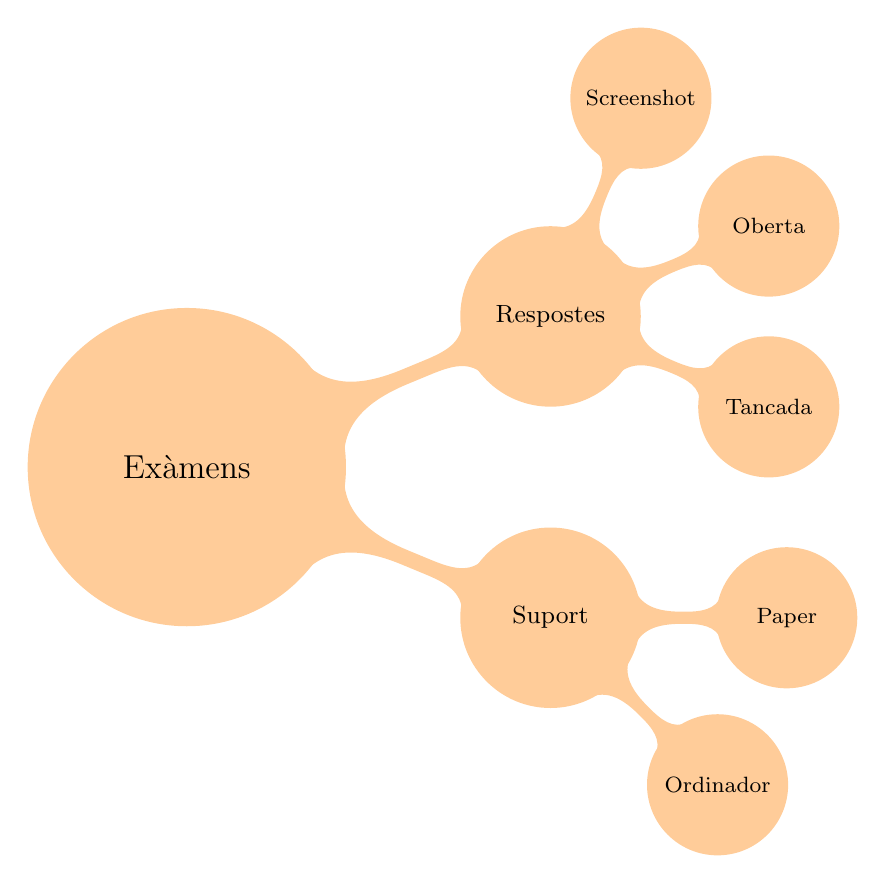
\begin{tikzpicture}[mindmap, grow cyclic, every node/.style=concept, concept color=orange!40, 
	level 1/.append style={level distance=5cm,sibling angle=45},
	level 2/.append style={level distance=3cm,sibling angle=45},]

\node{Exàmens}
	  child{ node {Suport}
	    child{ node {Ordinador}}
	    child{ node {Paper}}
	  }
	  child{ node {Respostes}
	    child{ node {Tancada}}
	    child{ node {Oberta}}
	    child{ node {Screenshot}}
	  }
;
\end{tikzpicture}
\caption{Classificació dels exàmens individuals segons el tipus de suport i el tipus de resposta.} \label{fig:M1}
\end{figure}

\section{Recursos materials}
TBD.

\section{Mesures per a l'atenció a la diversitat}
TBD.

\section{Connexió amb altres mòduls}
TBD.

\section{Elements transversals}
TBD.

\section{Unitats didàctiques}
TBD.

  \subsection{UD 1: Sistemes d'emmagatzemament de la informació.}
  TBD.

  \subsection{UD 2: Disseny lògic de bases de dades I. El model E-R.}
  TBD.

  \subsection{UD 3: Disseny lògic de bases de dades II. El model relacional.}
  TBD.

  \subsection{UD 4: Disseny físic de bases de dades I.}
  TBD.

  \subsection{UD 5: Disseny físic de bases de dades II. Gestió de taules.}
  TBD.

  \subsection{UD 6: Realització de consultes I.}
  TBD.

  \subsection{UD 7: Realització de consultes II. Subconsultes i consultes multitaula}
  TBD.

  \subsection{UD 8: Edició de les dades I.}
  TBD.

  \subsection{UD 9: Edició de les dades II. Dades relacionades i transaccions.}
  TBD.

  \subsection{UD 10: Guions I.}
  TBD.

  \subsection{UD 11: Guions II. Procediments, funcions, cursors.}
  TBD.

  \subsection{UD 12: Seguretat en les dades.}
  TBD.

\section{Conclusió}
TBD.

\section{Bibliografia}
TBD.

...

Això és una prova.
\end{document}
